\chapter{Exdeath's Castle}

\vspace{\baselineskip}

\begin{paracol}{2}

\begin{enumerate}
    \item Head to Exdeath's Castle
\end{enumerate}

\switchcolumn
\begin{misc}{Path to Exdeath's Castle}
    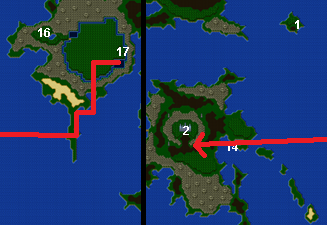
\includegraphics[scale=0.7]{../Graphics/Maps/12. To Exdeath's Castle.png}
\end{misc}

\switchcolumnTwice[*]
\begin{steproute}{Before Entering the Castle}
    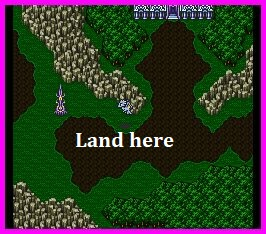
\includegraphics[scale=0.452]{../Graphics/Steps/158. Exdeath's Castle 1.jpg}
    \insertStep{../Graphics/Steps/159. Exdeath's Castle 2.jpg}
\end{steproute}

\switchcolumn
\begin{menu}{After the Half Step}
    \varwb
    \begin{jobMenu}
        \cara Ninja \textbf{(\pointLeft)(\pointDown)(\pointLeft)} \ability{\dash}
        \faris Mediator \textbf{(\pointUp)}       
    \end{jobMenu}
    \varwe
\end{menu}

\switchcolumnTwice[*]
\begin{enumerate}[resume]
    \item On the 2nd screen post transformation, activate the top left lever to grab the \pickup{Ice Shield}
\end{enumerate}

\switchcolumn
\begin{steproute}{MagicDragon}
    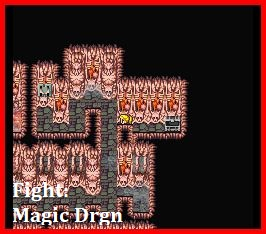
\includegraphics[scale=0.452]{../Graphics/Steps/160. Exdeath's Castle Enc 1.jpg}
\end{steproute}

\switchcolumn
\begin{encounter}{MagicDragon}
	\varwb
	\begin{notes}
		\item \encounterHl{Don't flee buffer}
	\end{notes}
	\begin{round}{1}
		\cara \leftCommand{\throw} \then \thunderScroll
        \bartz \rightCommand{\gilToss}
        \item \encounterHl{Be careful Lenna doesn't get her turn here}
        \faris \leftCommand{\catch}
	\end{round}
	\varwe
\end{encounter}

\switchcolumn
\begin{misc}{Menu Here}
    \insertScreenshot{../Graphics/Misc/17. Exdeath's Castle Menu.png}
\end{misc}

\switchcolumn
\begin{menu}{Before the Next Encounter}
    \varwb
    \begin{jobMenu}
        \faris Blue Mage \textbf{(\pointDown)(\pointLeft)(\pointDown)} \ability{!\gilToss}
        \begin{itemize}
            \item[] \equip{\iceShield}
        \end{itemize}
        \bartz Ninja \textbf{(\pointLeft)(\pointDown)(\pointLeft)} \ability{!\gilToss}
        \begin{itemize}
            \item[] \equip{\boneMail}
        \end{itemize}
        \lenna Blue Mage \textbf{(\pointDown)(\pointLeft)(\pointDown)} \ability{!\control}
        \begin{itemize}
            \item[] \optimize
        \end{itemize}
        \cara Mediator \textbf{(\pointUp)} \ability{\learning}
        \begin{itemize}
            \item[] \optimize
        \end{itemize}
    \end{jobMenu}
    \begin{itemMenu}
        \hiPotionMenu \ally{People missing 100+ HP}
    \end{itemMenu}
    \varwe
\end{menu}

\switchcolumn*
\begin{steproute}{MagicDragon, DarkWizard, TwinLizard}
    \insertStep{../Graphics/Steps/161. Exdeath's Castle Enc 2.jpg}
\end{steproute}

\switchcolumn
\begin{encounter}{MagicDragon, DarkWizard, TwinLizard}
	\varwb
	\begin{notes}
		\item \encounterHl{Don't flee buffer}
		\item \encounterHl{Make sure someone is hit by L.2 Old}
	\end{notes}
	\begin{round}{1}
		\bartz \leftCommand{\throw} \then \thunderScroll
        \cara Defend
        \faris Defend
        \lenna \rightCommand{\control} \then \enemy{MagicDragon}
	\end{round}
    \begin{round}{2}
		\bartz Defend
        \cara Defend
        \faris Defend
        \lenna \ltwoOld
        \item \encounterHl{Make sure it hits before continuing}
	\end{round}
    \begin{round}{3}
		\bartz Wait for L.2 Old cast \then \rightCommand{\gilToss}
        \cara \leftCommand{\catch}
	\end{round}
	\varwe
\end{encounter}

\switchcolumnTwice[*]
\begin{menu}{After the Encounter}
    \varwb
    \begin{jobMenu}
        \lenna Knight \textbf{(A)}
        \bartz Chemist \textbf{(\pointUp)(\pointRight)} \ability{!\gilToss}
        \begin{itemize}
            \item[] \optimize \space \then \unequip{Weapon}
        \end{itemize}
        \cara Thief \textbf{(2\pointRight)} \ability{!\escape}
    \end{jobMenu}
    \varwe
\end{menu}

\switchcolumn
\begin{steproute}{Before the Ether Chest}
    \insertStep{../Graphics/Steps/162. Exdeath's Castle 3.jpg}
\end{steproute}

\switchcolumn
\begin{enumerate}[resume]
    \item Grab the \pickup{Ether} chest on the screen after the encounters
    \item \battleGroup{Escape is the right command}
\end{enumerate}

\switchcolumn
\begin{steproute}{Before Exdeath}
    \insertStep{../Graphics/Steps/163. Exdeath's Castle Enc 3.jpg}
    \insertStep{../Graphics/Steps/164. Exdeath's Castle 4.jpg}
    \insertStep{../Graphics/Steps/165. Exdeath's Castle 5.jpg}
    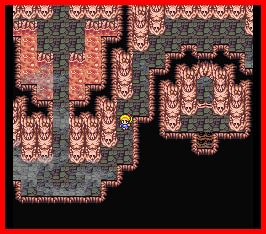
\includegraphics[scale=0.449]{../Graphics/Steps/166. Exdeath's Castle Enc 4.jpeg}
    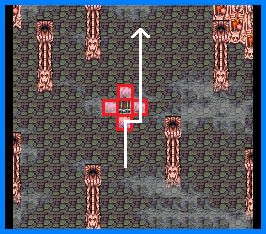
\includegraphics[scale=0.449]{../Graphics/Steps/167. Exdeath's Castle 6.jpeg}
    \insertStep{../Graphics/Steps/168. Exdeath's Castle 7.jpg}
\end{steproute}

\switchcolumn
\begin{menu}{Before Exdeath}
    \varwb
    \begin{jobMenu}
        \cara Blue Mage \textbf{(\pointDown)(\pointLeft)(\pointDown)} \ability{\dash} \optimize
    \end{jobMenu}
    \varwe
\end{menu}

\begin{boss}{Exdeath}
    \varwb
    \begin{round}{1}
        \cara \leftCommand{\blue} \then \ltwoOld
        \item \bossHl{Wait for 9 total "Can't run!!" messages}
        \item \bossNote{Have him selected and input when you see the 9th message disappear}
        \faris \leftCommand{\blue} \then \lfiveDeath
    \end{round}
    \varwe
\end{boss}

\end{paracol}